\section{Vom Problem zum Programm \verweis{1.2}}
	\subsection{Algorithmus}
		Der Begriff Programm ist eng mit dem Begriff Algorithmus verbunden. Algorithmen sind Vorschriften für die Lösung eines Problemes, welches die Handlungen und ihre Abfolge, also die Handlungsweise, beschreiben. Abstrakt kann man sagen, dass die folgenden Bestandteile und Eigenschaften zu einem Algorithmus gehören: \textit{(am Beispiel eines Kochrezeptes erklärt)} 
		\begin{compactitem}
			\item eine \textbf{Menge von Objekten}, die durch den Algorithmus bearbeitet werden \textit{(Zutaten, Geschirr, Herd, \dots)}
			\item eine \textbf{Menge von Operationen}, die auf den Objekten ausgeführt werden \textit{(waschen, schälen, \dots)}
			\item ein \textbf{definierter Anfangszustand}, in dem sich die Objekte zu Beginn befinden \textit{(Teller leer, Herd kalt, \dots)}
			\item ein \textbf{gewünschter Endzustand}, in dem sich die Objekte nach der Lösung des Problems befinden sollen \textit{(gekochtes Gemüse, \dots)}
		\end{compactitem}	

	\subsection{Der euklidische Algorithmus als Beispiel}
		\subsubsection{Das Problem}
				Eine rechteckige Terrasse sei mit möglichst grossen quadratischen Platten auszulegen. Welche Kantenlänge haben die Platten?
			
		\begin{minipage}[t]{9 cm}
			\subsubsection{Der Algorithmus}
				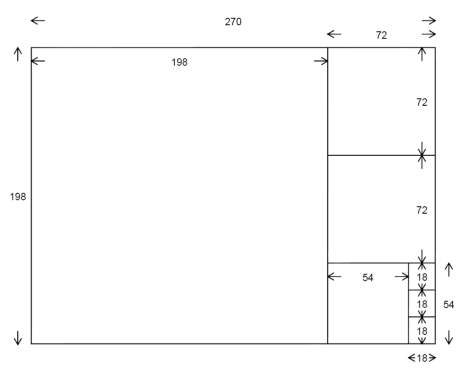
\includegraphics[width=1.0\textwidth]{pics/Euklid.jpg}
							
				Mit Abschneidetechnik nach Euklid. Entspricht der \\
				Ermittlung des grössten gemeinsamen Teilers (ggT): \\
				$\frac{x_{ungek"urzt}}{y_{ungek"urzt}}=\frac{\frac{x_{ungek"urzt}}{ggT(x_{ungek"urzt},y_{ungek"urzt})}}{\frac{y_{ungek"urzt}}{ggT(x_{ungek"urzt},y_{ungek"urzt})}}=\frac{x_{gek"urzt}}{y_{gek"urzt}}$ \\
					
			\subsubsection{Algorithmus-Beschreibung mit Struktogramm \verweis{1.3}}
				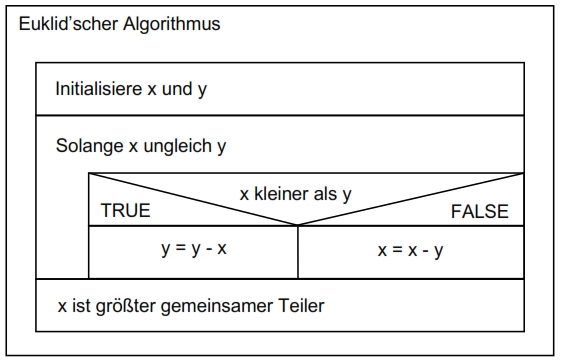
\includegraphics[width=1.0\textwidth]{pics/Euklid_Struktogramm.jpg}

		\end{minipage}
		%
		\begin{minipage}[t]{9 cm}	
			\subsubsection{Algorithmus-Beschreibung mit Pseudocode \verweis{1.2.1}}
				\lstinputlisting[language=C,tabsize=2]{code/Euklid_Pseudo.c}
					
				\subsubsection{Programm}
					\lstinputlisting[language=C,tabsize=2]{code/Euklid.c}
							
				\subsubsection{Trace-Tabelle \verweis{1.2.4}}
					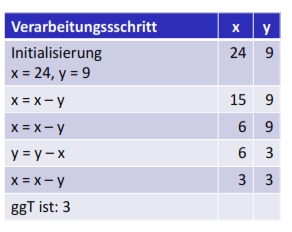
\includegraphics[width=0.58\textwidth]{pics/Euklid_Trace.jpg}
	
		\end{minipage}
		
	\subsection{Nassi-Shneiderman-Diagramme \verweis{1.3}}
		Zur Visualisierung des Kontrollflusses von Programmen, das heisst, zur grafischen Veranschaulichung ihres Ablaufes, wurden 1973 von Nassi und Shneiderman grafische Strukturen, die sogenannten Struktogramme, vorgeschlagen. Entwirft man Programme mit Nassi-Shneiderman-Diagrammen, so genügt man automatisch den Regeln der Strukturierten Programmierung.
		
		\begin{minipage}[t]{6 cm}
			\subsubsection{Sequenz}
				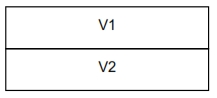
\includegraphics[width=1\textwidth]{pics/Nassi_Sequenz.jpg}
				
			\subsubsection{Block}
				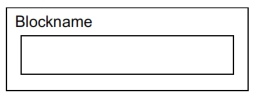
\includegraphics[width=1\textwidth]{pics/Nassi_Block.jpg}	
					
			\subsubsection{Einfache Alternative}
				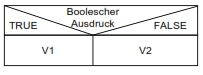
\includegraphics[width=1\textwidth]{pics/Nassi_einfache_Alternative.jpg}
					
		\end{minipage}
		%
		\begin{minipage}[t]{6 cm}
			\subsubsection{Bedingte Anweisung}
				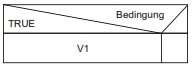
\includegraphics[width=1\textwidth]{pics/Nassi_bedingte_Verarbeitung.jpg}
								
			\subsubsection{Mehrfache Alternative}
				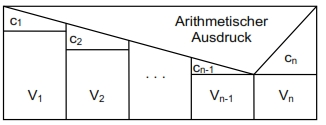
\includegraphics[width=1\textwidth]{pics/Nassi_mehrfache_Alternative.jpg}	
									
			\subsubsection{Schleife mit vorheriger Prüfung}
				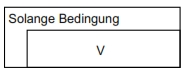
\includegraphics[width=1\textwidth]{pics/Nassi_While.jpg}
					
		\end{minipage}
		%
		\begin{minipage}[t]{6 cm}
			\subsubsection{Endlosschlaufe}
				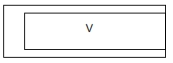
\includegraphics[width=1\textwidth]{pics/Nassi_While1.jpg}
											
			\subsubsection{Schleife mit nachfolgender Prüfung}
				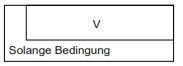
\includegraphics[width=1\textwidth]{pics/Nassi_DoWhile.jpg}	
					
			\subsubsection{Abbruchanweisung}
				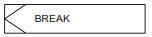
\includegraphics[width=1\textwidth]{pics/Nassi_Break.jpg}	
								
		\end{minipage}